\documentclass[a4j, 10pt, dvipdfmx, titlepage]{jarticle}
\usepackage[top=3cm, bottom=3cm, left=2.5cm, right=2.5cm]{geometry}
\usepackage[dvipdfmx]{graphicx}
\usepackage{bm}
\usepackage{float}
\usepackage{mathtools, amssymb}
\usepackage{color}
\usepackage{url}
\usepackage{pdfpages}


\usepackage{listings}
\usepackage{jlisting}

\lstset{
    language = C,
 	breaklines = true,
 	breakindent = 10pt,
 	basicstyle = \ttfamily\scriptsize,
 	classoffset = 0,
 	frame = tBRl,
 	framesep = 5pt,
 	numbers = left,
 	stepnumber = 1,
 	tabsize = 4,
 	captionpos = t
}
\renewcommand{\lstlistingname}{リスト}


\title{非公式プロコン競技プログラム仕様書}

\begin{document}
\mc{
    \maketitle
    \section{boardクラス}


        \begin{figure}[H]
            \centering
            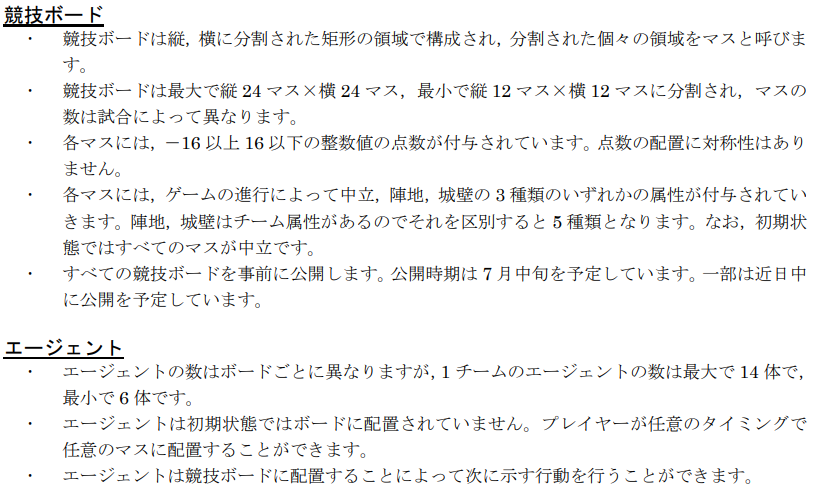
\includegraphics[scale=0.6]{memo_board.png}
            \caption{競技ボードの仕様(募集要項より)}
            \label{memoBoard}
        \end{figure}
        \begin{itemize}
            \item 定数
            \begin{enumerate}
                \item width $\cdots$ 
                \item height $\cdots$ ボードの高さ(12 - 24)
                \item agentNum $\cdots$ 各チームのエージェント数(6 - 14)
                \item fieldInfo $\cdots$ 盤面の地形情報 (自陣地, 自城壁, 中立, 敵陣地, 敵城壁)
                \item fieldPoint $\cdots$ 盤面の点数情報 (-16 - 16)
                \item agent $\cdots$ 盤面のエージェント情報
                \item Score $\cdots$ 両チームの得点情報
                \item agentCommand $\cdots$ エージェントの行動情報
            \end{enumerate}
            \item メンバ変数
            \begin{enumerate}
                \item width $\cdots$ ボードの幅(12 - 24)
                \item height $\cdots$ ボードの高さ(12 - 24)
                \item agentNum $\cdots$ 各チームのエージェント数(6 - 14)
                \item fieldInfo $\cdots$ 盤面の地形情報 (自陣地, 自城壁, 中立, 敵陣地, 敵城壁)
                \item fieldPoint $\cdots$ 盤面の点数情報 (-16 - 16)
                \item agent $\cdots$ 盤面のエージェント情報
                \item Score $\cdots$ 両チームの得点情報
                \item agentCommand $\cdots$ エージェントの行動情報
            \end{enumerate}
            \item 関数一覧
        \end{itemize}
}
\end{document}